Bộ Full Adder là một mạch logic số dùng để cộng 3-bit nhị phân, thường đầu vào được biểu diễn dưới dạng $A$, $B$, và $C_{in}$ (bit nhớ), đầu ra được biểu diễn dưới dạng $\text{SUM}(s)$ và $C_{out}$ (bit nhớ). Với $\text{SUM}(s) = A \oplus B \oplus C_{in}$ và $C_{out} = (A \& B) \| (C_{in} \& (A \oplus B))$.

\begin{figure}[H]
	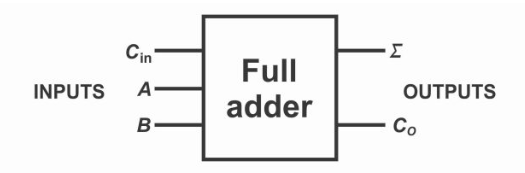
\includegraphics[width = 0.5\linewidth]{./image/full adder block.png}
	\centering
	\caption{Bộ Full Adder}
	\label{f_full adder block}	
\end{figure}

Bảng sự thật:

\begin{table}[H]
	\centering
	\begin{tabular}{|c|c|c|c|c|}
		\hline
		\multicolumn{3}{|c|}{Input} & \multicolumn{2}{c|}{Output}\\
		\hline
		$A$ & $B$ & $C_{in}$ & $\text{SUM}(s)$ & $C_{out}$\\
		\hline
		0 & 0 & 0 & 0 & 0\\
		\hline
		0 & 0 & 1 & 1 & 0\\
		\hline
		0 & 1 & 0 & 1 & 0\\
		\hline
		0 & 1 & 1 & 0 & 1\\
		\hline
		1 & 0 & 0 & 1 & 0\\
		\hline
		1 & 0 & 1 & 0 & 1\\
		\hline
		1 & 1 & 0 & 0 & 1\\
		\hline
		1 & 1 & 1 & 1 & 1\\
		\hline
	\end{tabular}
	\caption{Bảng sự thật của bộ Full Adder}
	\label{t_true table}
\end{table}

Thực hiện bộ Full Adder:

\begin{itemize}[label = -]
	\item Bộ Full Adder thực hiện bằng cổng logic:\\
		\begin{figure}[H]
			\centering
			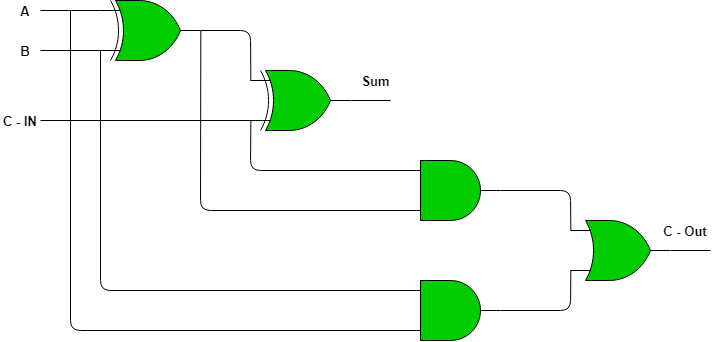
\includegraphics[width = .5\linewidth]{./image/full_adder_circuitcircuit.png}
			\caption{Bộ Full Adder thực hiện bằng cổng logic}
			\label{f_full adder circuit}
		\end{figure}
		
		\lstinputlisting[style=SystemVerilog, caption={Bộ Full Adder thực hiện bằng cổng logic}]{./code/full_adder/full_adder_circuit.sv}logic
	\item Bộ Full Adder thực hiện bằng bộ Half Adder:\\
		\begin{figure}[H]
			\centering
			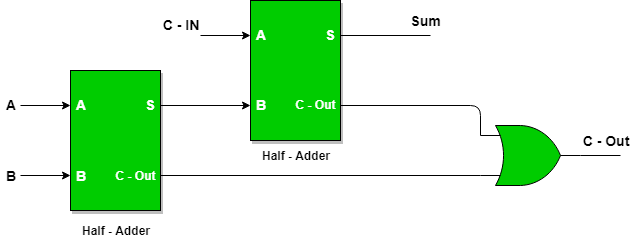
\includegraphics[width = 0.5\linewidth]{./image/full_adder_with_half_adder.png}
			\caption{Bộ Full Adder thực hiện bằng các bộ Half Adder}
			\label{f_full adder with half adder}
		\end{figure}
		
		\lstinputlisting[style=C, caption={Bộ Full Adder thực hiện bằng bộ Half Adder}]{./code/full_adder/full_adder_with_half_adder.sv}
\end{itemize}

Sử dụng các test case sau để kiểm tra hệ thống:

\begin{lstlisting}[style=C, caption={Test bench của bộ Full Adder}]
	#include <iostream>
	#include <verilated.h>
	#include "VName_moduel.h" // Verilator-generated header file
	
	int main(int argc, char **argv) {
		// Initialize Verilator
		Verilated::commandArgs(argc, argv);
		
		// Create an instance of the module
		VName_moduel* dut = new VName_moduel;
		
		// Input test vectors
		int test_cases[8][3] = {
			{0, 0, 0}, // {i_data_a, i_data_b, i_carry}
			{0, 0, 1},
			{0, 1, 0},
			{0, 1, 1},
			{1, 0, 0},
			{1, 0, 1},
			{1, 1, 0},
			{1, 1, 1},
		};
		
		// Print table header
		std::cout << "A B Cin | Sum Cou" << std::endl;
		std::cout << "--------|--------" << std::endl;
		
		// Run test cases
		for (int i = 0; i < 8; ++i) {
			// Apply inputs
			dut->i_data_a = test_cases[i][0];
			dut->i_data_b = test_cases[i][1];
			dut->i_carry  = test_cases[i][2];
			
			// Evaluate the circuit
			dut->eval();
			
			// Display inputs and outputs
			std::cout << test_cases[i][0] << " "
			<< test_cases[i][1] << "   "
			<< test_cases[i][2] << "  |   "
			<< (int)dut->o_data << "   "
			<< (int)dut->o_carry << std::endl;
		}
		
		// Cleanup
		delete dut;
		
		return 0;
	}
\end{lstlisting}

Kết quả:

\begin{lstlisting}[style=C, caption={Kết quả của test bench của bộ Full Adder sử dụng cổng logic}]
	$ ./obj_dir/Vfull_adder_circuit 
	A B Cin | Sum Cou
	--------|--------
	0 0   0  |   0   0
	0 0   1  |   1   0
	0 1   0  |   1   0
	0 1   1  |   0   1
	1 0   0  |   1   0
	1 0   1  |   0   1
	1 1   0  |   0   1
	1 1   1  |   1   1
\end{lstlisting}


\begin{lstlisting}[style=C, caption={Kết quả của test bench của bộ Full Adder sử dụng bộ Half Adder}]
	$ ./obj_dir/Vfull_adder_with_half_adder 
	A B Cin | Sum Cou
	--------|--------
	0 0   0  |   0   0
	0 0   1  |   1   0
	0 1   0  |   1   0
	0 1   1  |   0   1
	1 0   0  |   1   0
	1 0   1  |   0   1
	1 1   0  |   0   1
	1 1   1  |   1   1
\end{lstlisting}